\documentclass[12pt,answers]{exam}

\usepackage[margin=0.5in]{geometry}
\usepackage{amsmath,amssymb}
\usepackage{tikz,soul}
\usepackage{diagbox}
\usepackage{pmboxdraw}
\usetikzlibrary{arrows,automata,positioning}

\newcommand{\ds}{\displaystyle}
\newcommand{\bs}{\backslash}
\newcommand{\on}{\operatorname}
\newcommand{\R}{\mathbb{R}}
\newcommand{\Z}{\mathbb{Z}}
\newcommand{\N}{\mathbb{N}}

\begin{document}
\pagestyle{empty}
\subsubsection*{Homework 7 - Computer Science 461 \hfill Name: \underline{\hspace*{2in}}}

\textit{Due Monday, March 24.} % You can e-mail your code for the computer programming problems to me at }\verb|blins@hsc.edu|.

\begin{questions}

\question Use the algorithm we discussed in class (see the notes from Wed, March 5) to convert the following context-free grammar to Chomsky normal form:
% NOTE TO SELF: I DIDN'T DO THIS PROBLEM IN CLASS, BUT IF YOU HAVE USED IT, THEN MODIFY THIS EXERCISE!

\begin{minipage}{1.5in}
\begin{align*}
S &\rightarrow ASA ~|~ A ~|~ \epsilon \\
A &\rightarrow aa ~|~ \epsilon \\
\end{align*}
\end{minipage}

\begin{solution}
\begin{description}
\item[Add new start variable.] $S_0 \rightarrow S ~|~ \epsilon$.
\item[Remove epsilon rules.] $S \rightarrow AS ~|~ SA ~|~ASA  ~|~ A$ and $A \rightarrow aa$. 
\item[Remove unit rules.] $S \rightarrow AS ~|~ SA ~|~ASA  ~|~ aa$. 
\item[Add terminal variables.] $A \rightarrow T_a T_a$ and $T_a \rightarrow a$.
\item[Break up long rules.] $S \rightarrow AS ~|~ SA ~|~ AU ~|~ aa$ where $U \rightarrow SA$. 
\end{description} 

So the grammar in Chomsky normal form is:
\begin{align*}
S_0 &\rightarrow S ~|~ \epsilon \\
S &\rightarrow AS ~|~ SA ~|~ AU ~|~ T_a T_a\\
A &\rightarrow T_a T_a \\
U &\rightarrow SA \\
T_a &\rightarrow a 
\end{align*}

\end{solution}
\vfill


\question Give a detailed written description (but not a state diagram) of a Turing machine that accepts the following language.
$$L = \{ w \in \{a,b\}^* : w \text{ has an equal number of }a\text{'s and }b\text{'s} \}.$$

\begin{solution}
\textbf{Option 1.} Use a section of the tape to store an encoding of an integer which is initially 0.  Move left to right through the input reading either $a$ or $b$.  If you get an $a$, then replace with an $x$ and then move to the integer and increase it by one.  If you get a $b$, replace it with an $x$ and decrease the integer by 1.  When there are no more $a$s and $b$s, move to the integer and accept if it is zero and reject otherwise. \\
 
\textbf{Option 2.} Reading left to right, if you see an $a$, then replace it with an $x$, then move right until you see a $b$.  If you find one replace it with an $x$ too, but if you get to a blank first, reject.  If you see a $b$ replace it with an $x$, then more right until you get to an $a$.  Replace it with an $x$, or reject if you get to a blank first.  If you see an $x$ ignore it, and move right.  

After this, move all the way to the left and then repeat.  If you get to a blank without seeing either an $a$ or $b$, then accept. 
\end{solution}
\vfill

%\question Give a detailed written description (but not a state diagram) of a Turing machine that accepts the following languages.
%\begin{parts}
%\part $L = \{ w \in \{a,b\}^* : w \text{ has an equal number of }a\text{'s and }b\text{'s} \}$.
%\begin{solution}
%%Use a section of the tape to store an encoding of an integer which is initially 0.  Move left to right through the input reading either $a$ or $b$.  If you get an $a$, then replace with an $x$ and then move to the integer and increase it by one.  If you get a $b$, replace it with an $x$ and decrease the integer by 1.  When there are no more $a$s and $b$s, move to the integer and accept if it is zero and reject otherwise.  
%Reading left to right, if you see an $a$, then replace it with an $x$, then move right until you see a $b$.  If you find one replace it with an $x$ too, but if you get to a blank first, reject.  If you see a $b$ replace it with an $x$, then more right until you get to an $a$.  Replace it with an $x$, or reject if you get to a blank first.  If you see an $x$ ignore it, and move right.  
%
%After this, move all the way to the left and then repeat.  If you get to a blank without seeing either an $a$ or $b$, then accept. 
%\end{solution}
%
%\vfill
%
%\part $L = \{a^n b^{2n} c^{3n} : n \ge 1 \}$. 
%\begin{solution}
%Moving left to right, when you see an $a$ replace with an $x$, then  move right until you see a $b$. Replace two $b$'s with an $x$ if you can (otherwise reject), then move right until you see a $c$. Replace the next three $c$'s with $x$'s (if you can, otherwise reject).  Then move left to leftmost $a$ and repeat.  If there are no $a$'s remaining, move right and check that there are no $b$'s and $c$'s and accept iff there are none.
%\end{solution}
%\vfill
%\end{parts}

%\question Let $\Sigma = \{a\}$. Draw a state diagram for a Turing machine that evaluates the function $f:\Sigma^* \rightarrow \Sigma^*$ defined by $f(a^n) = a^{2n}$.  
%\vfill

%\question Describe an algorithm for a Turing machine that computes the function $f(a^n) = a^{2n}$. 
%\vfill

\question A \verb|binary-incrementer| is a function that reads a binary number from a tape, and replaces it with the binary number that is one greater.  So 111 becomes 1000, for example.  Draw a state diagram for a Turing machine that evaluates the \verb|binary-incrementer| function. Hint: You should only need a few states.  
\begin{solution}
\begin{center}
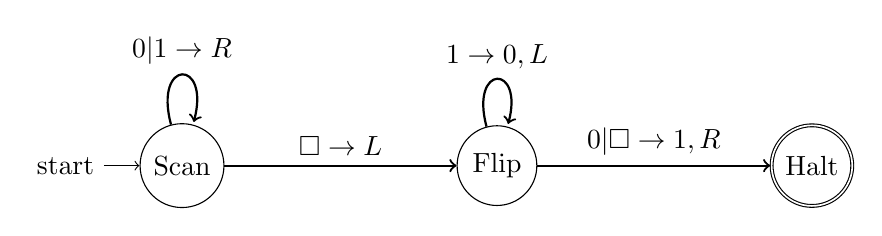
\begin{tikzpicture}[node distance=4cm,auto]
  \node[state,initial]   (q_1)                 {Scan};
  \node[state]           (q_2) [right of=q_1]  {Flip};
  \node[state,accepting]           (q_3) [right of=q_2]  {Halt};
  \path[thick,->]
  (q_1) edge [loop above] node {$0|1 \rightarrow R$} (q_1)
  (q_1) edge              node {$\square \rightarrow L$} (q_2)
  (q_2) edge              node {$0|\square \rightarrow 1,R$} (q_3)
  (q_2) edge [loop above] node {$1 \rightarrow 0,L$} ();
\end{tikzpicture}
\end{center}
\end{solution}
\vfill

\newpage
\question If you have a Turing machine that computes the \verb|binary-incrementer| function, explain how you could create a Turing machine that reads a string of $n$ 1's, and replaces it with the binary integer that represents $n$. For example 1111 would become 100 since 100 represents $n=4$ in binary. %Hint: In your description you can use a separator character to separate the string of 1's from the binary output. 
You don't need to draw a state diagram, but explain in detail how you would incorporate the \verb|binary-incrementer| machine into your new Turing machine.
\begin{solution}
Add a separator symbol and a 0 to left of input.  The read the input right to left replacing each read 1 with a blank and then incrementing the binary number to the left of the separator.  Repeat until there is nothing right of the separator, then remove the separator.  
\end{solution}

\vfill

\question Let $\Sigma$ be an alphabet, and let $L \subset \Sigma^*$ be a language.  If $L$ is decidable, prove that its complement $\overline{L}$ is also decidable. 
\begin{solution}
Let $D$ be a decider for $L$.  Create a new TM $E$ that accepts $w$ if $D$ rejects $w$ and rejects $w$ when $D$ accepts $w$. Then $E$ is a decider for $\overline{L}$. 
\end{solution}

\vfill

\question Why doesn't the same argument show that the complement of an acceptable language is acceptable?  
\begin{solution}
If we only have a recognizer $R$ for $L$, then $R$ may loop forever on some strings.  So we wouldn't know whether that string is in $L$ or in $\overline{L}$. 
\end{solution}
\vfill

%\question Explain why the following description is not enough to describe a Turing machine:
%
%For a tape with input representing a polynomial (i.e., \verb|3x^2+5x+7|),
%\begin{enumerate}
%\item Set the value of the variable $x$ to every possible integer value. 
%\item Evaluate the polynomial at these values of $x$.
%\item Accept the string if it ever evaluates to zero, otherwise reject. 
%\end{enumerate}
%\vfill  % ACTUALLY, THE PROBLEM LIKE THIS IN SIPSER APPEARS TO WANT TO HIGHLIGHT THE "OTHERWISE REJECT" STATEMENT, NOT THE FACT THAT ALL OF THE DETAILS OF HOW THE TM RUNS ARE NOT INCLUDED. 

\end{questions}
\end{document}
